\chapter{Design}\label{design}

The following chapter describes the details concerning the design process of the system.

The whole process was carried out with a step-by-step approach, starting from the design of the visual language and early prototypes of the development environment, proceeding with the storage backend, and finally concluding with the integration with the execution backend.

Specifically, the design of the visual language and the development of the web-based IDE prototypes were carried out iteratively, in order to adopt a PDCA (Plan-Do-Check-Act) approach.
The latter allowed receiving realistic feedback straight away, thus intercepting potential problems early on and speeding up the entire process.

Due to the hard time constraint of the internship and to obtain ease of use, although sometimes trading off with expressivity, only a core subset of \moise{} features were implemented.
This also implies that the system was not designed as a complete replacement of \moise{}, but rather as a tool to facilitate the use of this technology also by users with no programming skills.

Moreover, as some parts of the system were designed knowing that they might need a full project focused only on them, this project leaves space for future improvements and integrations, such as the implementation of the remaining features and the exploitation of different technologies.

\section{A Visual Language for Organizations}\label{visual-language}
The main challenge in this project is surely the design of a visual language that, on one hand, is expressive enough to represent the organizational structure and the goals of an organization, and, on the other hand, is easy to use and understand by non-technical users.

Since the visual abstractions are the main artifact of the system, the design of the language was the first step of the project and has gone through several iterations, possibly even evolving further in the future thanks to feedback from real users.

\subsection{The Visual Paradigm}
The choice of the most suitable visual paradigm was the first step of the design process since it is crucial to define the overall look and feel of the language.
Indeed, it is of fundamental importance to choose a paradigm that is easy to use, allows the users to easily understand the meaning of the visual abstractions, is coherent with the concepts to represent, and can be easily translated into the actual specification.

Comparing the existing paradigms for visual programming, the most natural choice was the diagram-based paradigm.
Other approaches, even though already proven to be effective in many fields, were not perfectly suitable for this purpose.
For instance, flow-based programming better fits the modeling of the way data must flow during the execution of the program, while block-based programming is more suitable to describe instructions to be executed in an imperative programming style.

On the other hand, the diagram-based paradigm is appropriate to specify the characteristics of a system in a declarative programming fashion, therefore being highly convenient for the definition of an organizational specification.

\subsection{Reference Language}
To facilitate the design of the visual language, it was necessary to study and understand the organization specification language in order to identify the ``building blocks'' that could be used to represent the organizational structure and the goals of an organization.
Since, as already mentioned, the system has \moise{} as a strong constraint and reference, as the organization specifications created should be compliant with it, the \moise{} language was chosen as a reference.

The analysis of the concepts and the syntax of the reference language, to be ported as visual elements, first involved looking at the \moise{} XML metamodel that defines the rules for the organization specification syntax.
A few examples of the main constructs are shown in \cref{lst:xml-metamodel}\footnote{The entire metamodel can be found at \url{https://github.com/moise-lang/moise/blob/master/src/main/resources/xml/os.xsd}}.

As can be observed, a role definition requires the specification of an attribute \texttt{id}, that is the name of the role, and it may specify some roles it extends from through \texttt{extends} children elements.
On the other hand, a goal definition requires the specification of the attributes \texttt{id}, that is the name of the goal, \texttt{ds}, that is the description, etc. and it may specify arguments, dependencies from other goals, and plans, with \texttt{argument}, \texttt{depends-on}, and \texttt{plan} children elements, respectively.

\begin{figure}[H]
    \lstinputlisting[language=XML,label={lst:xml-metamodel},caption={\moise{} syntax rules for the XML specification of roles and goals.}]{code/moise-metamodel.xsd}
\end{figure}

The actual syntax used in the XML organization specification for roles and goals definition can be found in \cref{lst:xml-model}.
As can be observed, there are two roles defined, \texttt{role1} and \texttt{role2}, with the latter extending from the former.
As far as the goals are concerned, there are four of them in total; the goal \texttt{goal2} has a description, the argument \texttt{arg1}, depends on the goal \texttt{goal1} and has a plan that consists of the sequence of the two goals \texttt{goal3} and \texttt{goal4}, that is $g2 = g3,g4$.

\begin{figure}[H]
    \lstinputlisting[language=XML,label={lst:xml-model},caption={\moise{} actual sintax for the XML specification of roles and goals.}]{code/moise-model.xml}
\end{figure}

Moreover, since a graphical representation of some of the \moise{} constructs is already available, it was possible to use them as a reference and starting point for the design of the visual language.

\begin{figure}[H]
    \begin{subfigure}[h]{0.4\linewidth}
        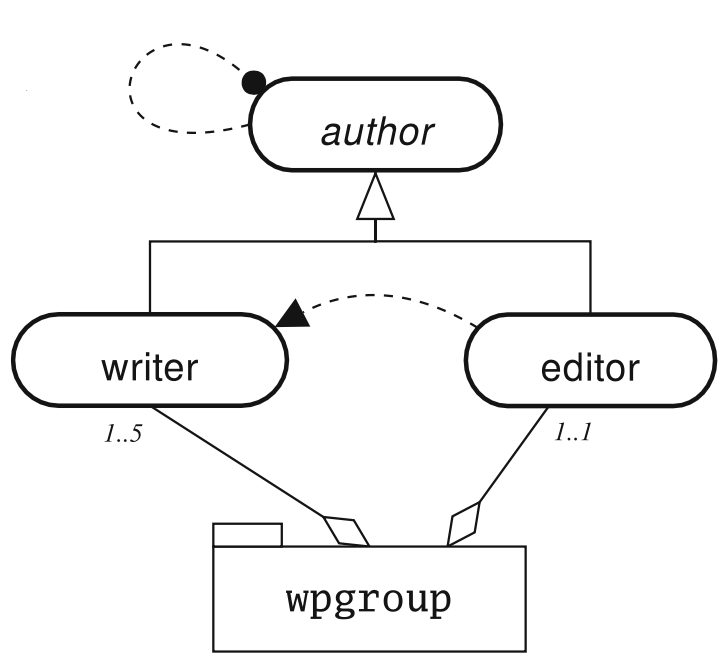
\includegraphics[width=\textwidth]{images/moise-structural.png}
        \caption{Structural specification}
        \label{fig:moise-structural}
    \end{subfigure}
    \begin{subfigure}[h]{0.6\linewidth}
        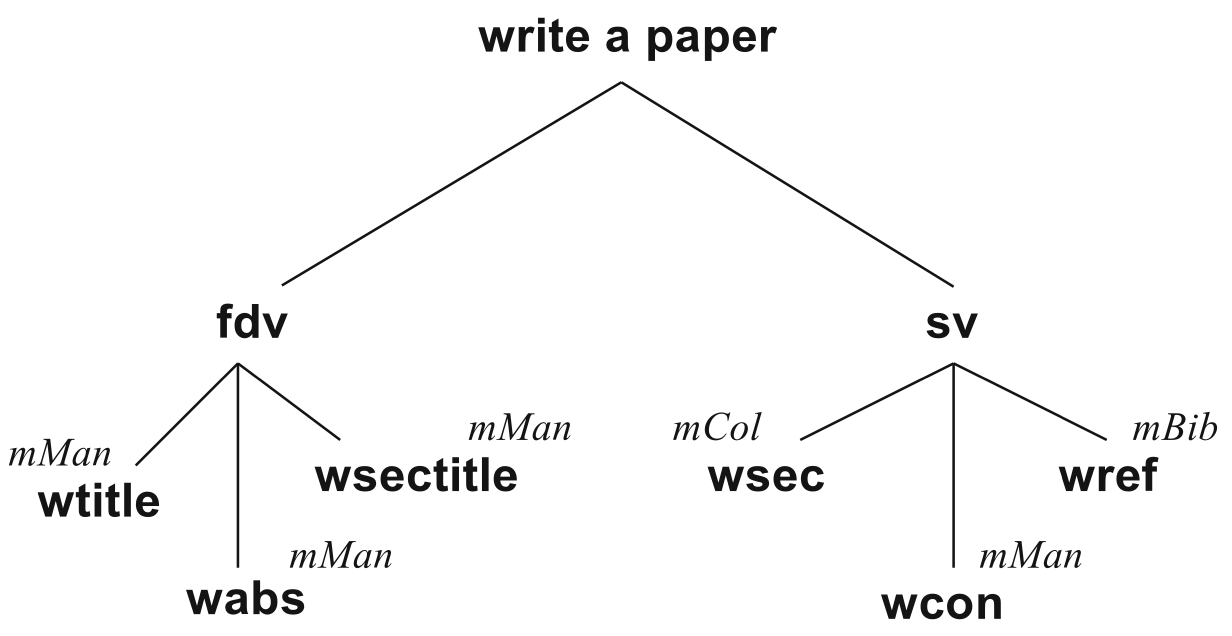
\includegraphics[width=\textwidth]{images/moise-functional.png}
        \caption{Functional specification}
        \label{fig:moise-functional}
    \end{subfigure}
    \caption{Visual representation of the structural and functional specification in \moise{}. Adopted from~\cite{hubner2010}.}
    \label{fig:moise-visual}
\end{figure}

The scenario described in \cref{fig:moise-visual} considers agents that aim at writing a paper and therefore have to collaborate.

As shown in \cref{fig:moise-structural}, the structure of the organization has only one group, that is the \texttt{wpgroup} represented by a folder, with two roles defined, \texttt{writer} and \texttt{editor} represented by rounded rectangles, that extend, and therefore inherit the properties of, the \texttt{author} role.
The relations and links among roles and groups are represented by arrows, with the pattern of the line and the different harrow heads indicating the type of relation.
Indeed, a solid line with an empty diamond head indicates that the role is a member of a group, i.e. \texttt{writer} and \texttt{editor} are members of the \texttt{wpgroup} group.
On the other hand, a solid line with an empty harrow head indicates that the source role extends the target role, i.e. \texttt{writer} and \texttt{editor} extend the \texttt{author} role.
Moreover, a dashed line with a round head indicates that the source role can communicate with the target role, i.e. \texttt{author} can communicate with \texttt{author}, which in this scenario means that every agent can communicate with every other agent.
Finally, a dashed line with a filled harrow head indicates that the source has authority on the target, i.e. \texttt{editor} has authority on \texttt{writer}.

As far as the functional specification shown in \cref{fig:moise-functional} is concerned, the goals of the organization are represented in a tree-like structure, thus following the goal decomposition tree abstraction, with the root goal being the \texttt{write a paper} goal.
The latter is decomposed into two subgoals, \texttt{fdv} (first draft version) and \texttt{sv} (submission version), through a sequence plan.
What is more, the \texttt{fdv} and \texttt{sv} goals are decomposed through sequence plans into three subgoals each, that are \texttt{wtitle}, \texttt{wabs}, and \texttt{wsectitles} and \texttt{wsec}, \texttt{wcon}, and \texttt{wref}, respectively.
Therefore, the plans can be formalized as:
\begin{gather}
    \text{\texttt{write a paper}} = \text{\texttt{fdv}}, \text{\texttt{sv}} \nonumber\\
    \text{\texttt{fdv}} = \text{\texttt{wtitle}}, \text{\texttt{wabs}}, \text{\texttt{wsectitles}} \nonumber\\
    \text{\texttt{sv}} = \text{\texttt{wsec}}, \text{\texttt{wcon}}, \text{\texttt{wref}} \nonumber
\end{gather}

\section{Visual Language Design}
Once the main concepts were extrapolated both from a syntactical and semantic point of view and their visual representation was analyzed, the design process of the visual language started.

One of the first crucial decisions was to keep the structure and the behavior of the organization separate, as it is done in \moise{}.
This choice was made because it allows the user to focus on one aspect at a time, thus making them feel not overwhelmed by the complexity of the tool.
Moreover, it allows re-using some visual building blocks in both the structural and the functional specification with a different meaning, thus reducing the number of elements that the user has to learn.

Thereafter, the main components of the core concepts of the visual language were defined.
As already mentioned, their design followed an iterative design process that made them more and more refined thanks to the feedback from the user tests.

\subsection{Structure of the Organization}
In this section, the visual representation of the main concepts regarding the structure of the organization are described.
As already mentioned, the structure and the behavior of the organization are modeled separately using two different diagrams, therefore the following visual elements will be used in the structural specification diagram.

\subsubsection{Roles}
The roles of the organization are represented by circles, with the name of the role written above them.
As can be seen in \cref{fig:roles}, the concrete roles are represented by a solid circle, while the abstract roles are represented by an empty circle.

\begin{figure}[H]
    \begin{subfigure}[h]{0.5\linewidth}
        \begin{center}
            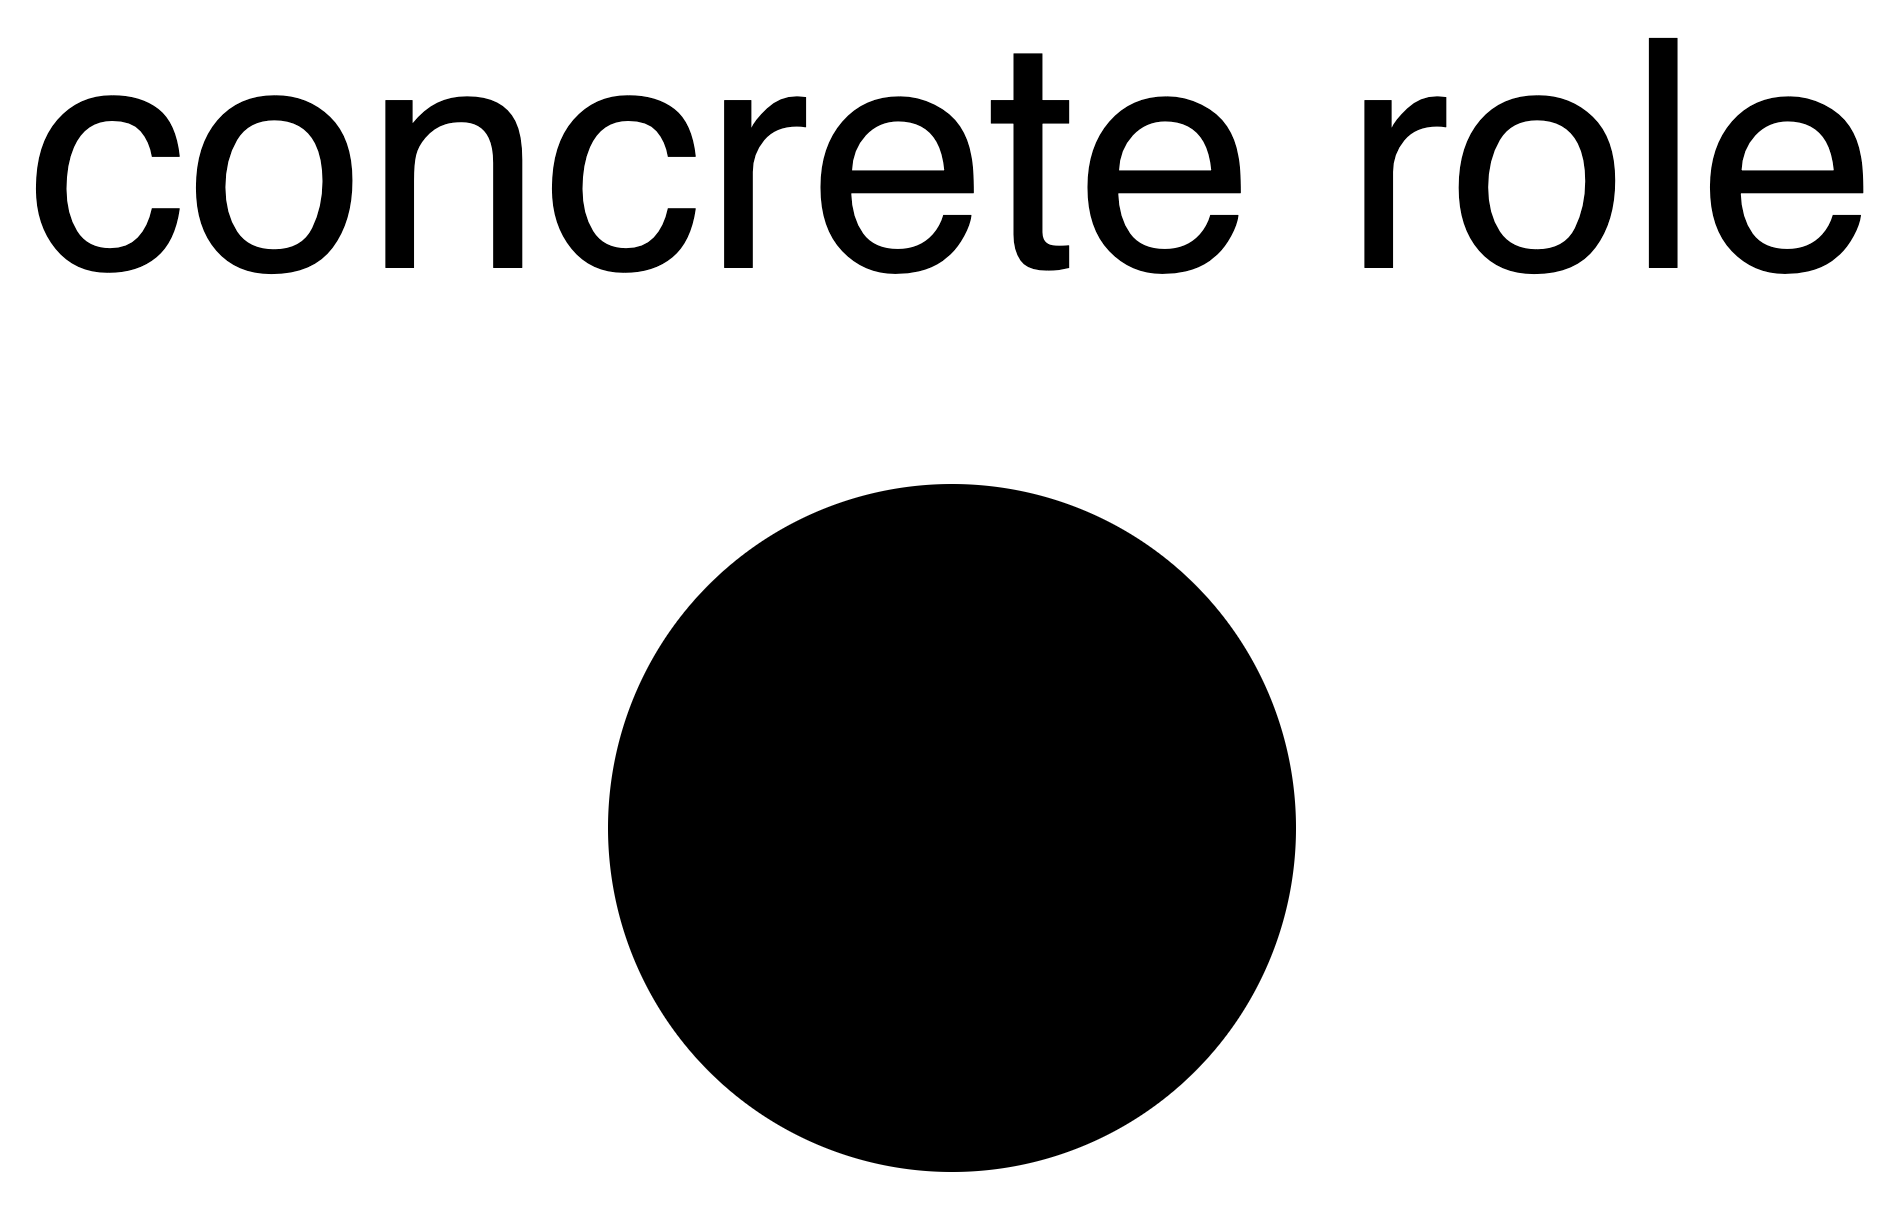
\includegraphics[width=0.5\textwidth]{images/visual-language/concrete-role.png}
            \caption{Representation of a concrete role.}
            \label{fig:concrete-role}
        \end{center}
    \end{subfigure}
    \begin{subfigure}[h]{0.5\linewidth}
        \begin{center}
            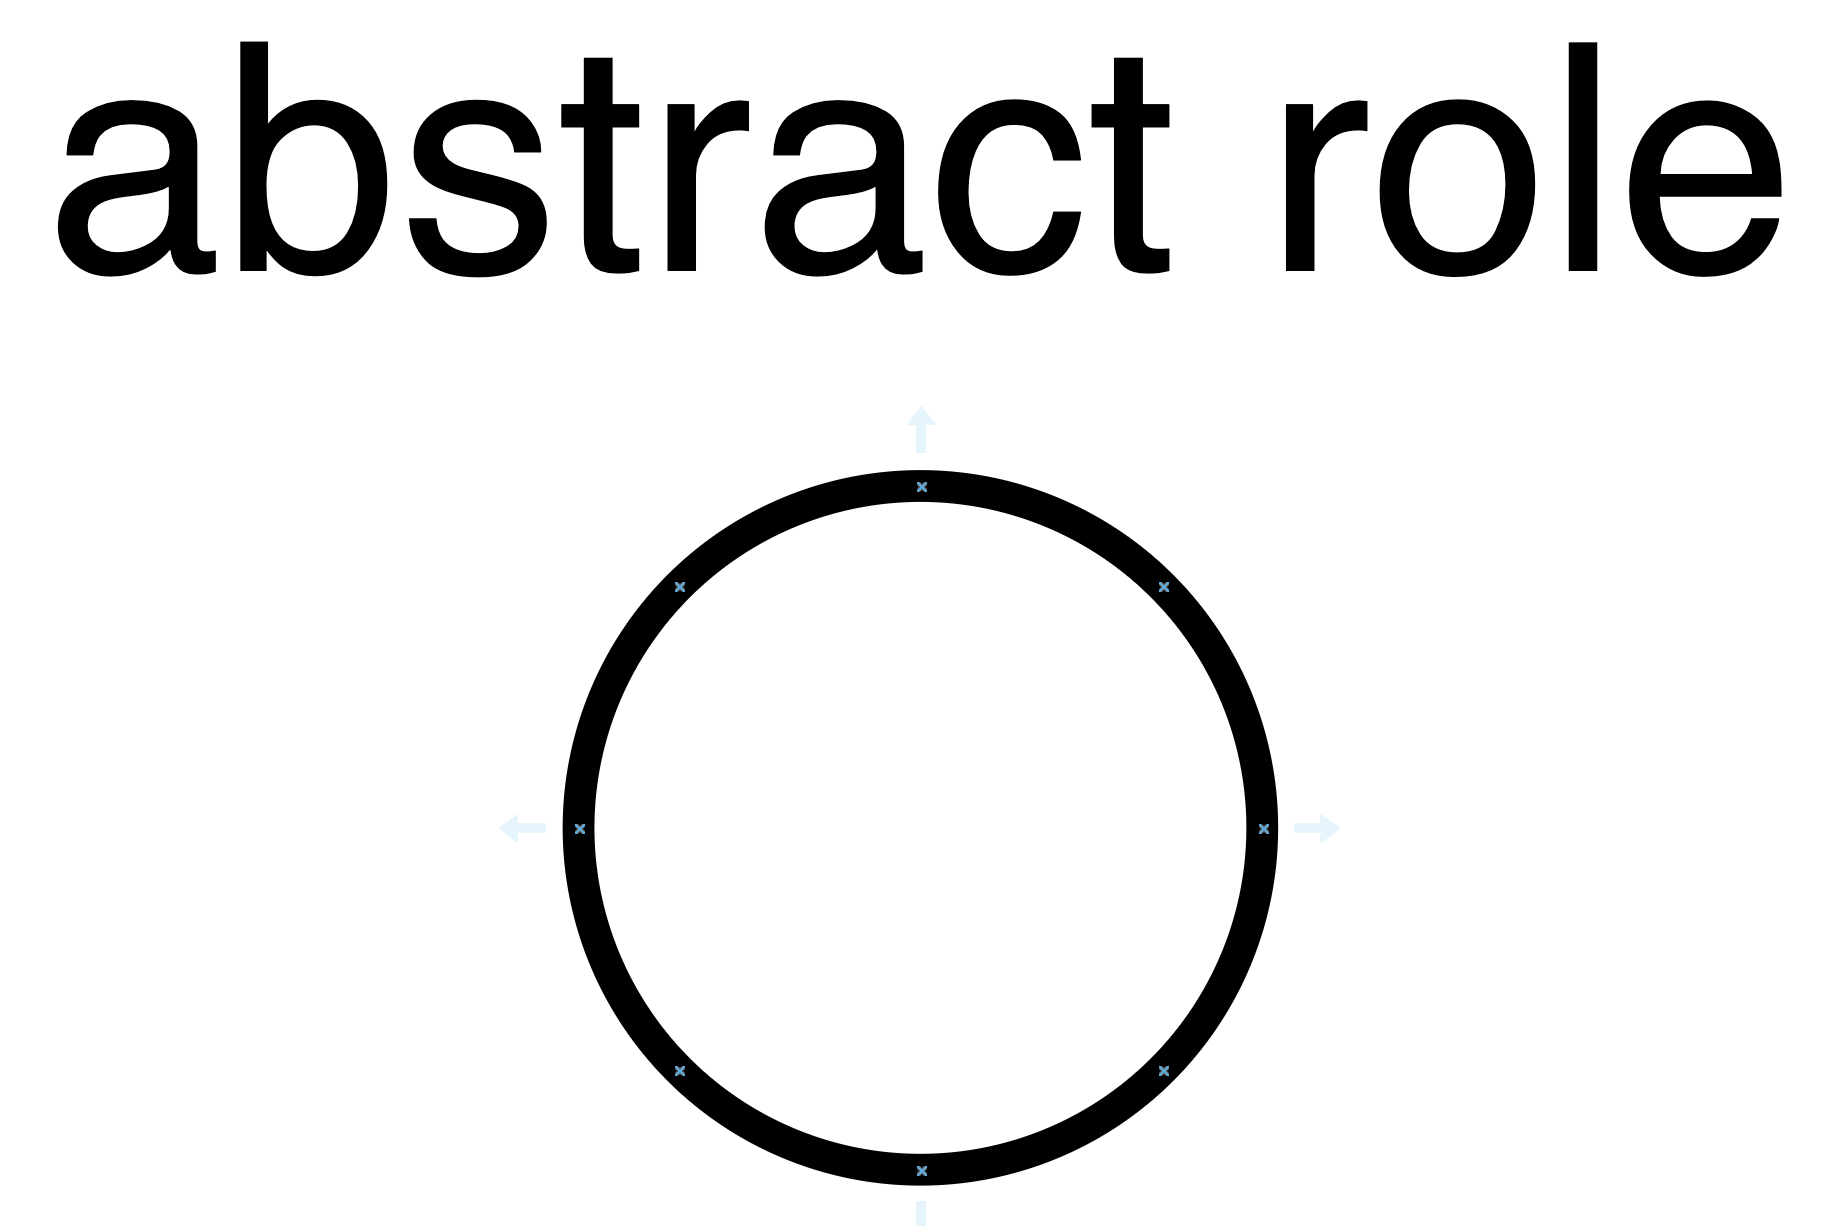
\includegraphics[width=0.5\textwidth]{images/visual-language/abstract-role.png}
            \caption{Representation of an abstract role.}
            \label{fig:abstract-role}
        \end{center}
    \end{subfigure}
    \caption{Roles representation in the visual language.}
    \label{fig:roles}
\end{figure}

The introduction of the abstract roles was made to allow the user to define a role that is not directly played by an agent or part of a group, but that can be extended by other roles.
This is useful and powerful when the user wants to define some common properties that are shared by more roles, thus avoiding the repetition of the same properties in the different roles.
For instance, such roles could be assigned goals, links, constraints, etc. that are then inherited by the roles that extend them, in a similar way to the abstract classes inheritance in object-oriented programming.
Moreover, the visual diversification between concrete and abstract roles emphasizes the difference between the two concepts, thus making the language more intuitive and suggesting the user this feature.

\subsubsection{Groups}
The groups of the organization are represented by rounded rectangles, with the name of the group written above them as shown in \cref{fig:group}.
This container-like shape was chosen to suggest to the user that elements such as roles and other groups can be placed inside it.
Therefore, the visual semantics of an element placed inside a group is that of membership, i.e. the element is a member of the group.

\begin{figure}[H]
    \centering
    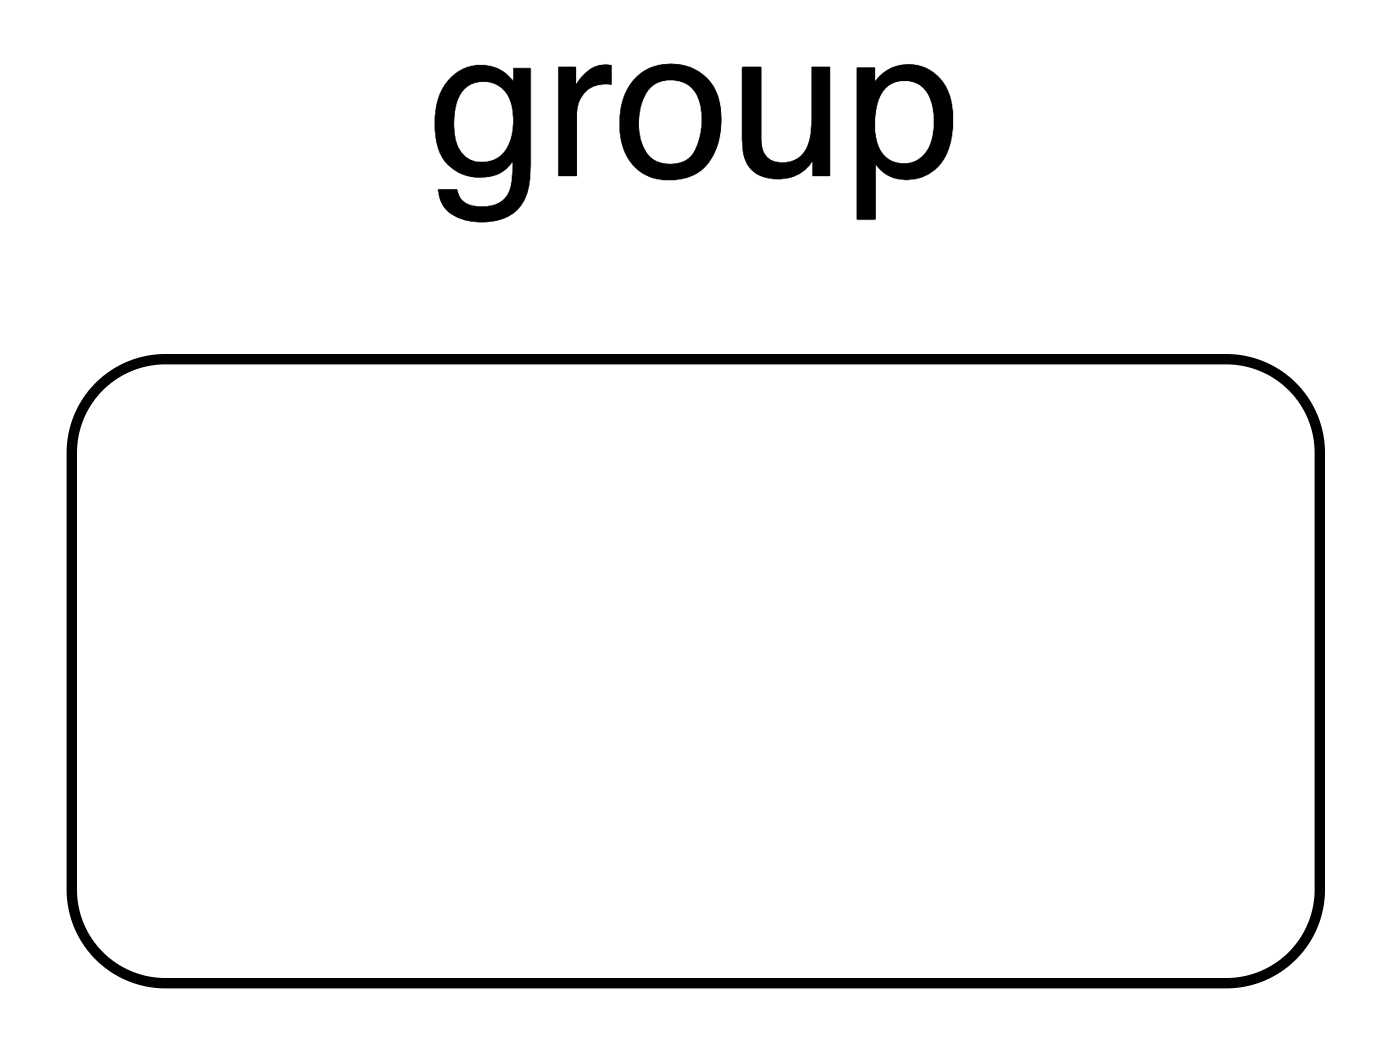
\includegraphics[width=0.3\linewidth]{images/visual-language/group.png}
    \caption{Representation of a group.}
    \label{fig:group}
\end{figure}

The elements that can be placed inside a group, and therefore be part of it, are the roles and other groups.

The choice to allow groups to be members of other groups was made to allow the user to define a hierarchy of groups, thus allowing them to define a more complex structure of the organization.
This is particularly powerful when a group is composed of multiple instances with the same structure, as it allows the user to define the subgroup structure only once, using it as a template to check the well-formedness of the instances.

As far as the roles are concerned, only the concrete roles can be members of a group, since, as already mentioned, the abstract roles are not directly played by an agent and therefore not part of a group.

In \cref{fig:groups} it is possible to see an example of a simple structure that exploits group hierarchies and the role membership concept.
In particular, the group \texttt{g1} is composed of the role \texttt{r1} and the group \texttt{g2}, which is composed of the role \texttt{r2}.
This shows how exploiting only two visual elements, i.e. the groups and the roles, it is possible to define rather complex structures.

\begin{figure}[H]
    \centering
    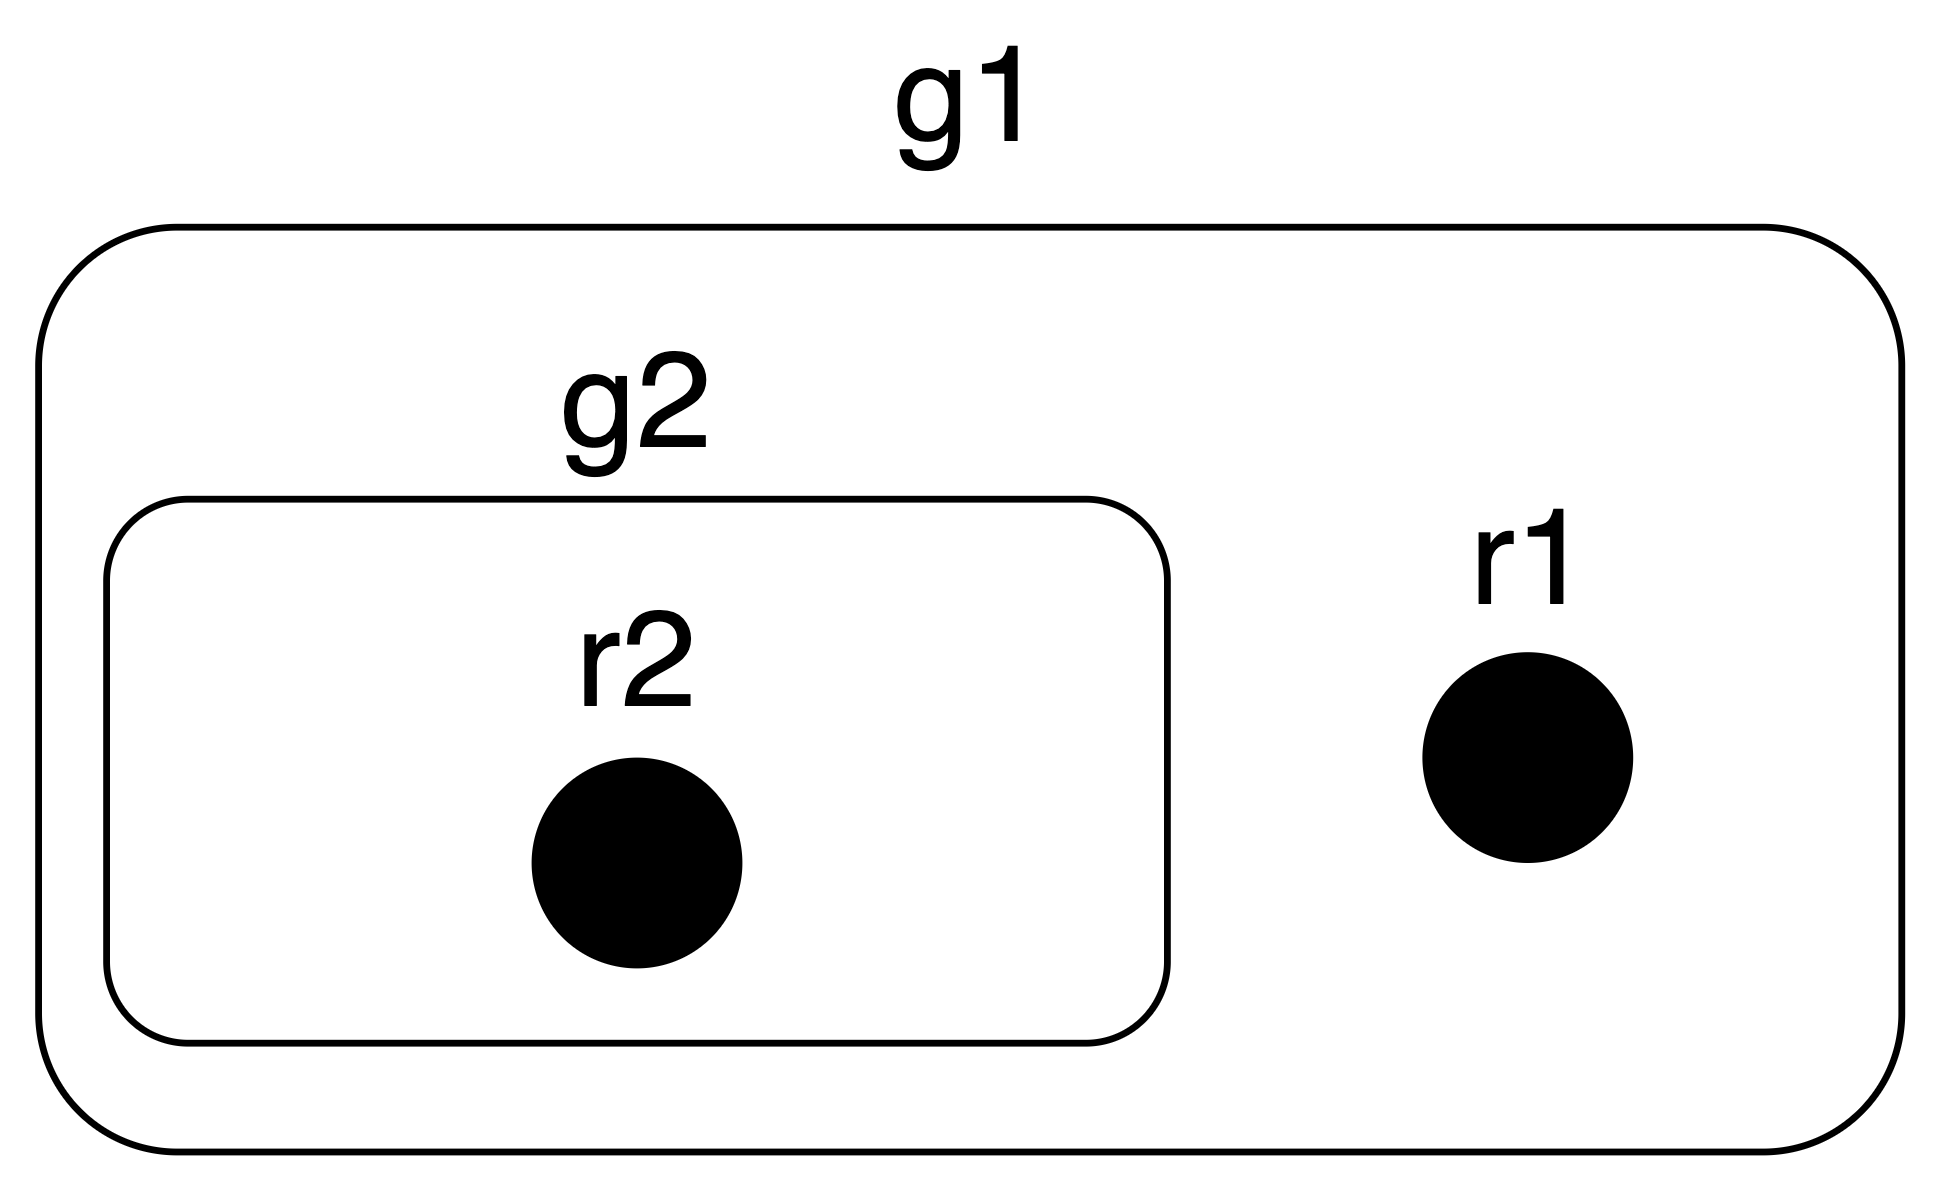
\includegraphics[width=0.5\linewidth]{images/visual-language/groups.png}
    \caption{Example of a structure that exploits group hierarchies and the role membership concept.}
    \label{fig:groups}
\end{figure}

\subsubsection{Relations}
The relations between the roles of the organization are represented by arrows, with the style of the arrow giving information about the type of relation.
Only a subset of the relations defined in \moise{} is currently represented and supported by the visual language since the others are either not used in practice or there is no way to enforce them in the current version of the JaCaMo framework.
Therefore, the core relations were identified and chosen, giving space to future work to extend the visual language to support the remaining relations.

\begin{figure}[H]
    \begin{subfigure}[h]{0.5\linewidth}
        \centering
        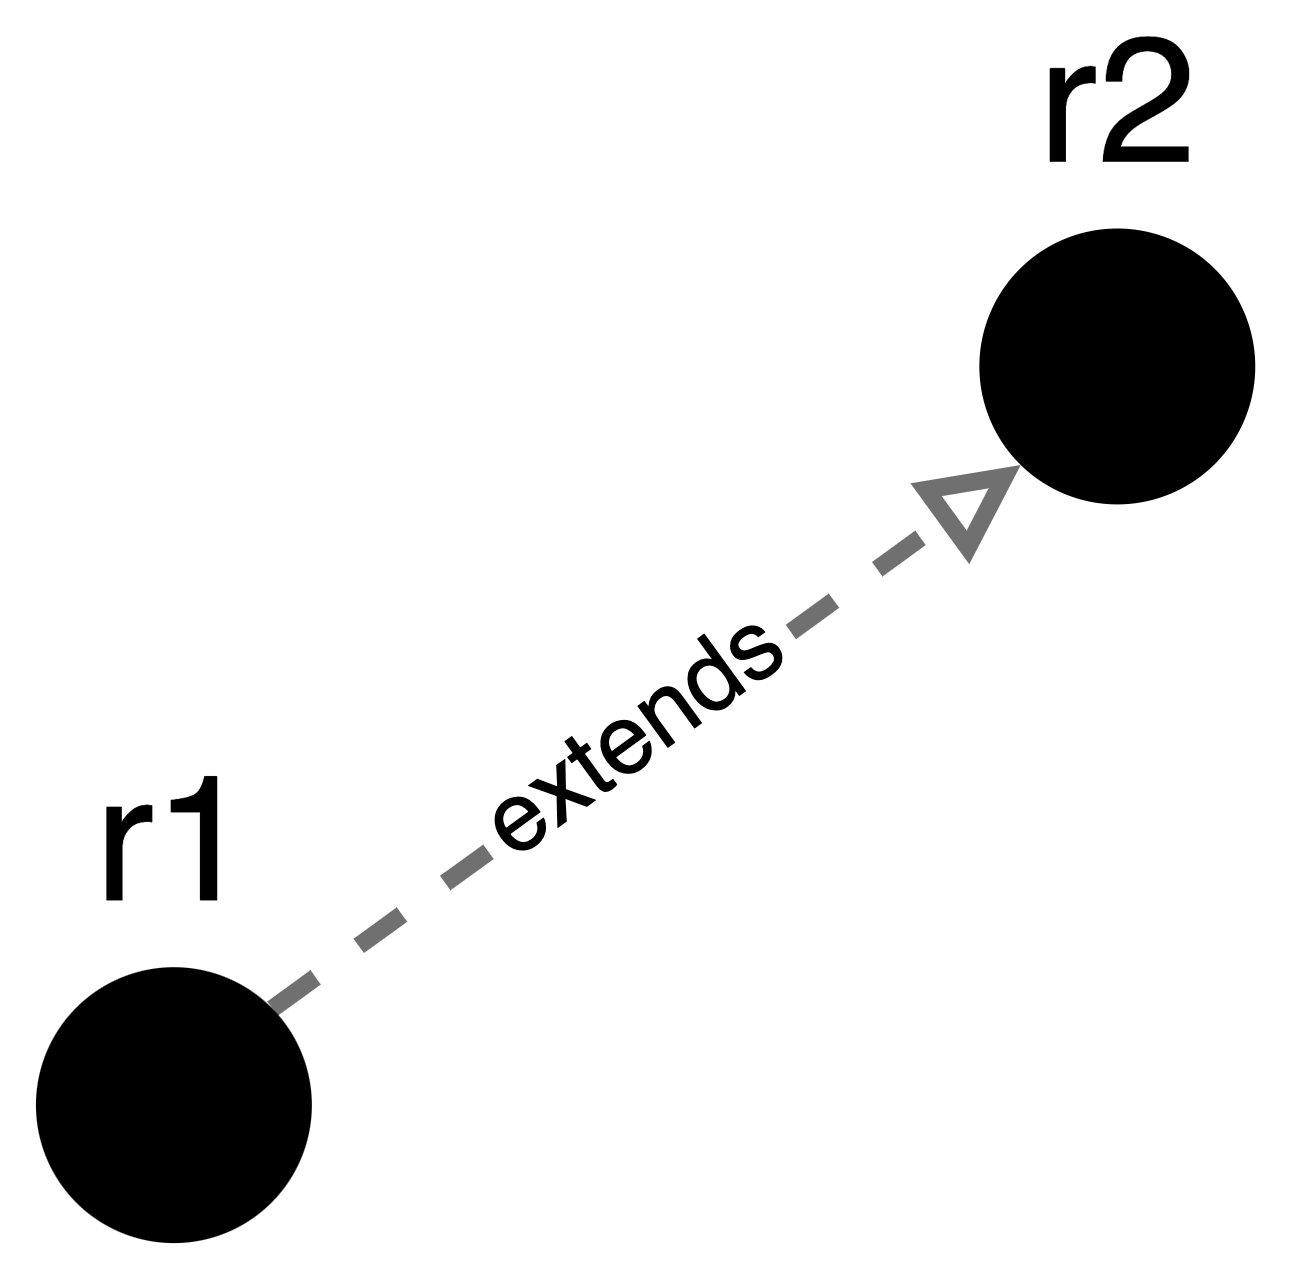
\includegraphics[width=0.5\textwidth]{images/visual-language/extension.png}
        \caption{Extension relation among roles.}
        \label{fig:extension}
    \end{subfigure}
    \begin{subfigure}[h]{0.5\linewidth}
        \centering
        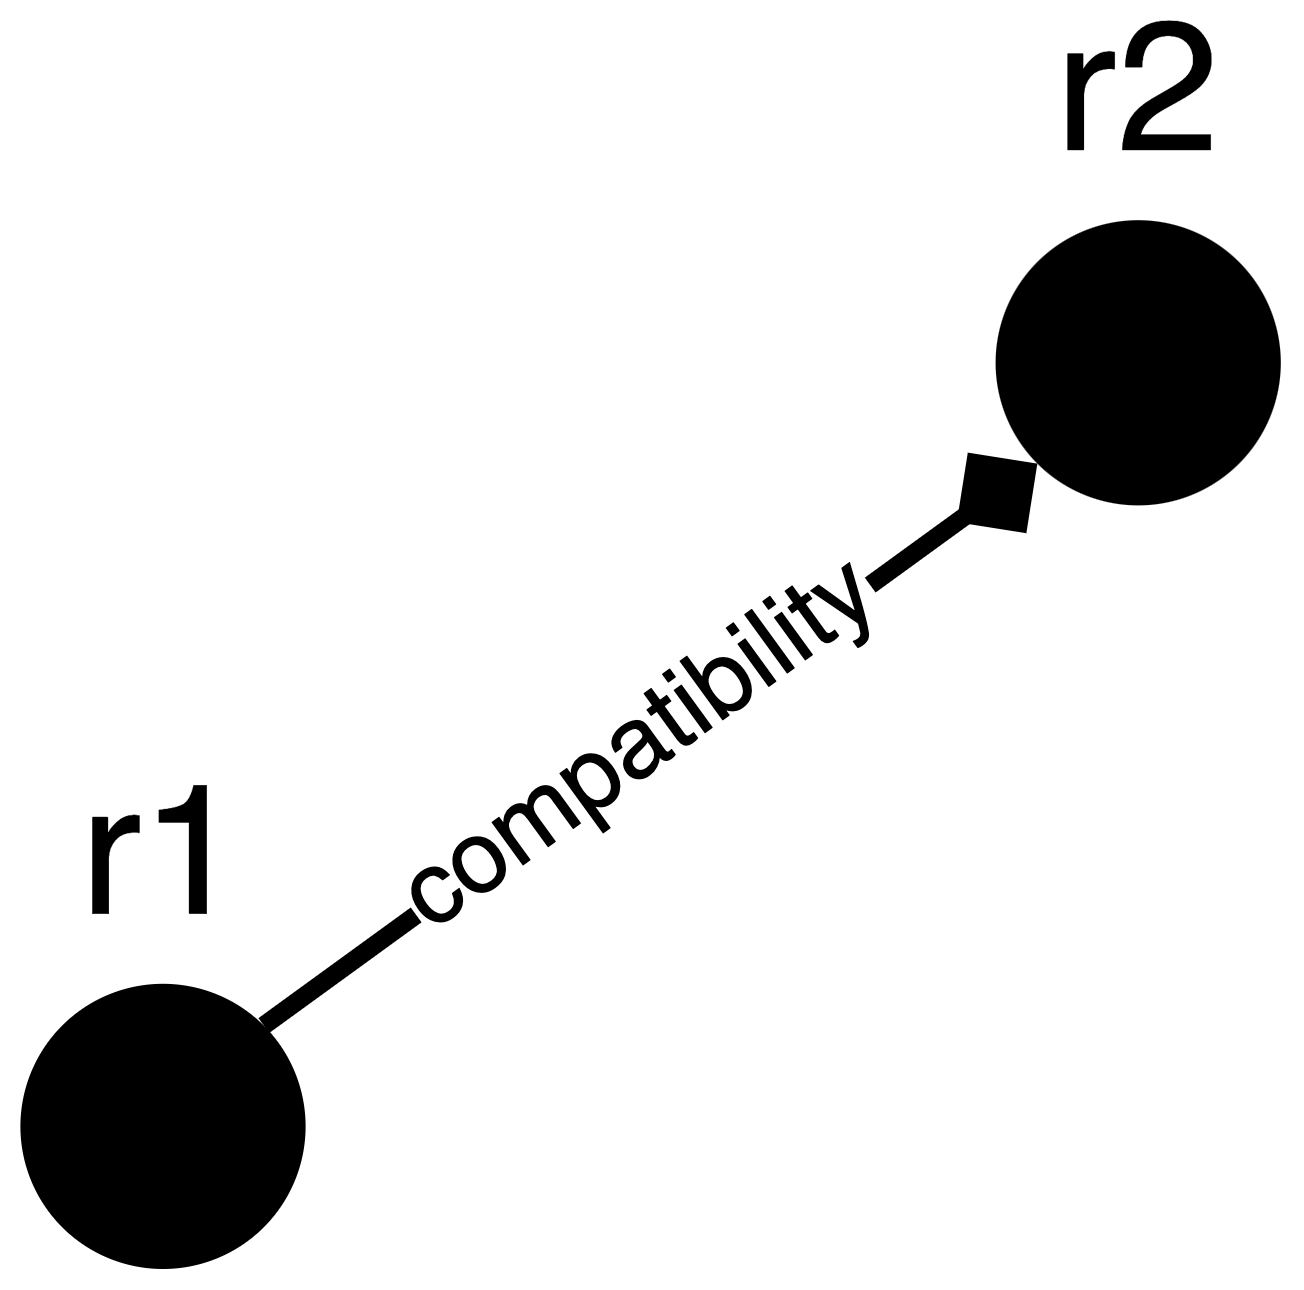
\includegraphics[width=0.5\textwidth]{images/visual-language/compatibility.png}
        \caption{Compatibility relation among roles.}
        \label{fig:compatibility}
    \end{subfigure}
    \caption{Visual representation of the implemented relations.}
    \label{fig:relations}
\end{figure}

As shown in \cref{fig:relations}, the subset of relations that are currently supported by the visual language are the extension and the compatibility relations.

The extension relation, visible in \cref{fig:extension}, is represented by an arrow with a dashed line, an empty harrow head, a slightly dimmed color, and the \texttt{extends} label on it.
In particular, the source role, i.e. \texttt{r1}, extends the target role, i.e. \texttt{r2}, meaning that the source role is a specialization of the target role.

On the other hand, the compatibility relation, depicted in \cref{fig:compatibility}, is represented by an arrow with a solid line, a filled diamond on the target end, a dark color, and the \texttt{compatibility} label on it.
In this scenario, the source role, i.e. \texttt{r1}, is compatible with the target role, i.e. \texttt{r2}, meaning that the target role can be played by an agent that is already playing the source role.

\subsection{Behavior of the Organization}
After describing the visual components of the organization structure, the next step is to present the visual abstractions that allow the user to define the behavior of the organization.
The following elements will be used in the functional specification diagram, therefore separated from the one regarding the structure.

\subsubsection{Goals}
The goals of the organization are represented by rectangles with rounded corners, with the name of the goal written inside them as shown in \cref{fig:goal}.

\begin{figure}[H]
    \centering
    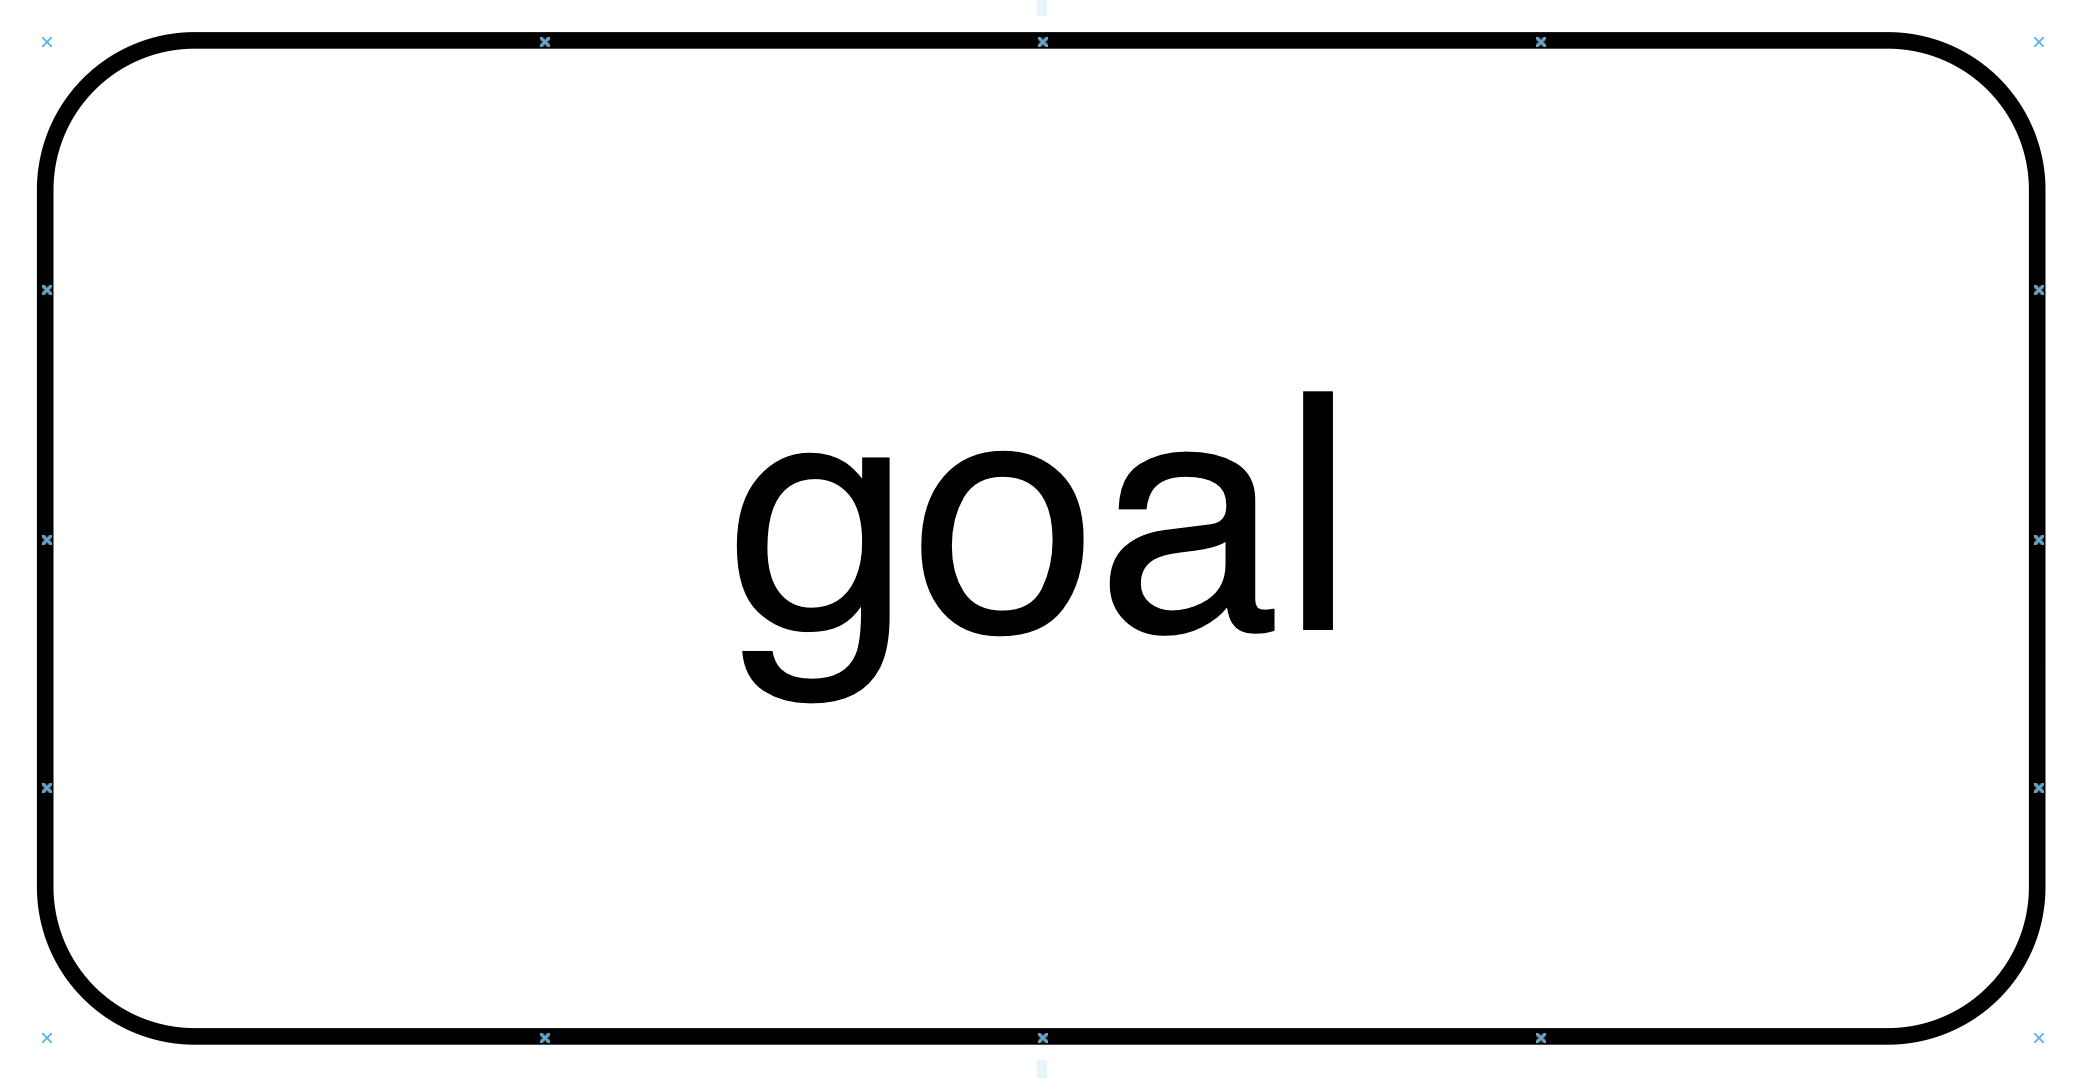
\includegraphics[width=0.3\linewidth]{images/visual-language/goal.png}
    \caption{Representation of a goal.}
    \label{fig:goal}
\end{figure}

Unlike the groups, the choice to place the label inside the rectangle was made to suggest to the user that the goal can be a complete element by itself.

Even though according to the \moise{} model a goal can be composed of multiple subgoals, representing them inside the supergoal rectangle would make the diagram too complex and hard to read, not to talk about the scalability issues that would arise.
Indeed, when defining complex scenarios, several levels of decomposition can be reached, and the multiple nesting of subgoals would make the diagram not understandable at first glance.

To address this issue, the choice was made to also represent the subgoals of a goal as top-level elements.
In this way, the user can still easily identify the subgoals of a goal, while the diagram stays readable and easy to understand.

Therefore, the decision was to diverge from the \moise{} model and represent the goals not as a goal decomposition tree but as a \textit{dependency graph}, where the nodes are the goals and the edges are the dependencies between them.

\subsubsection{Dependencies}
The dependencies between the goals of the organization are represented by arrows that connect goals, with the style of the arrow giving information about the type of dependency, as shown in \cref{fig:dependencies}.

\begin{figure}[H]
    \begin{subfigure}[h]{0.5\linewidth}
        \centering
        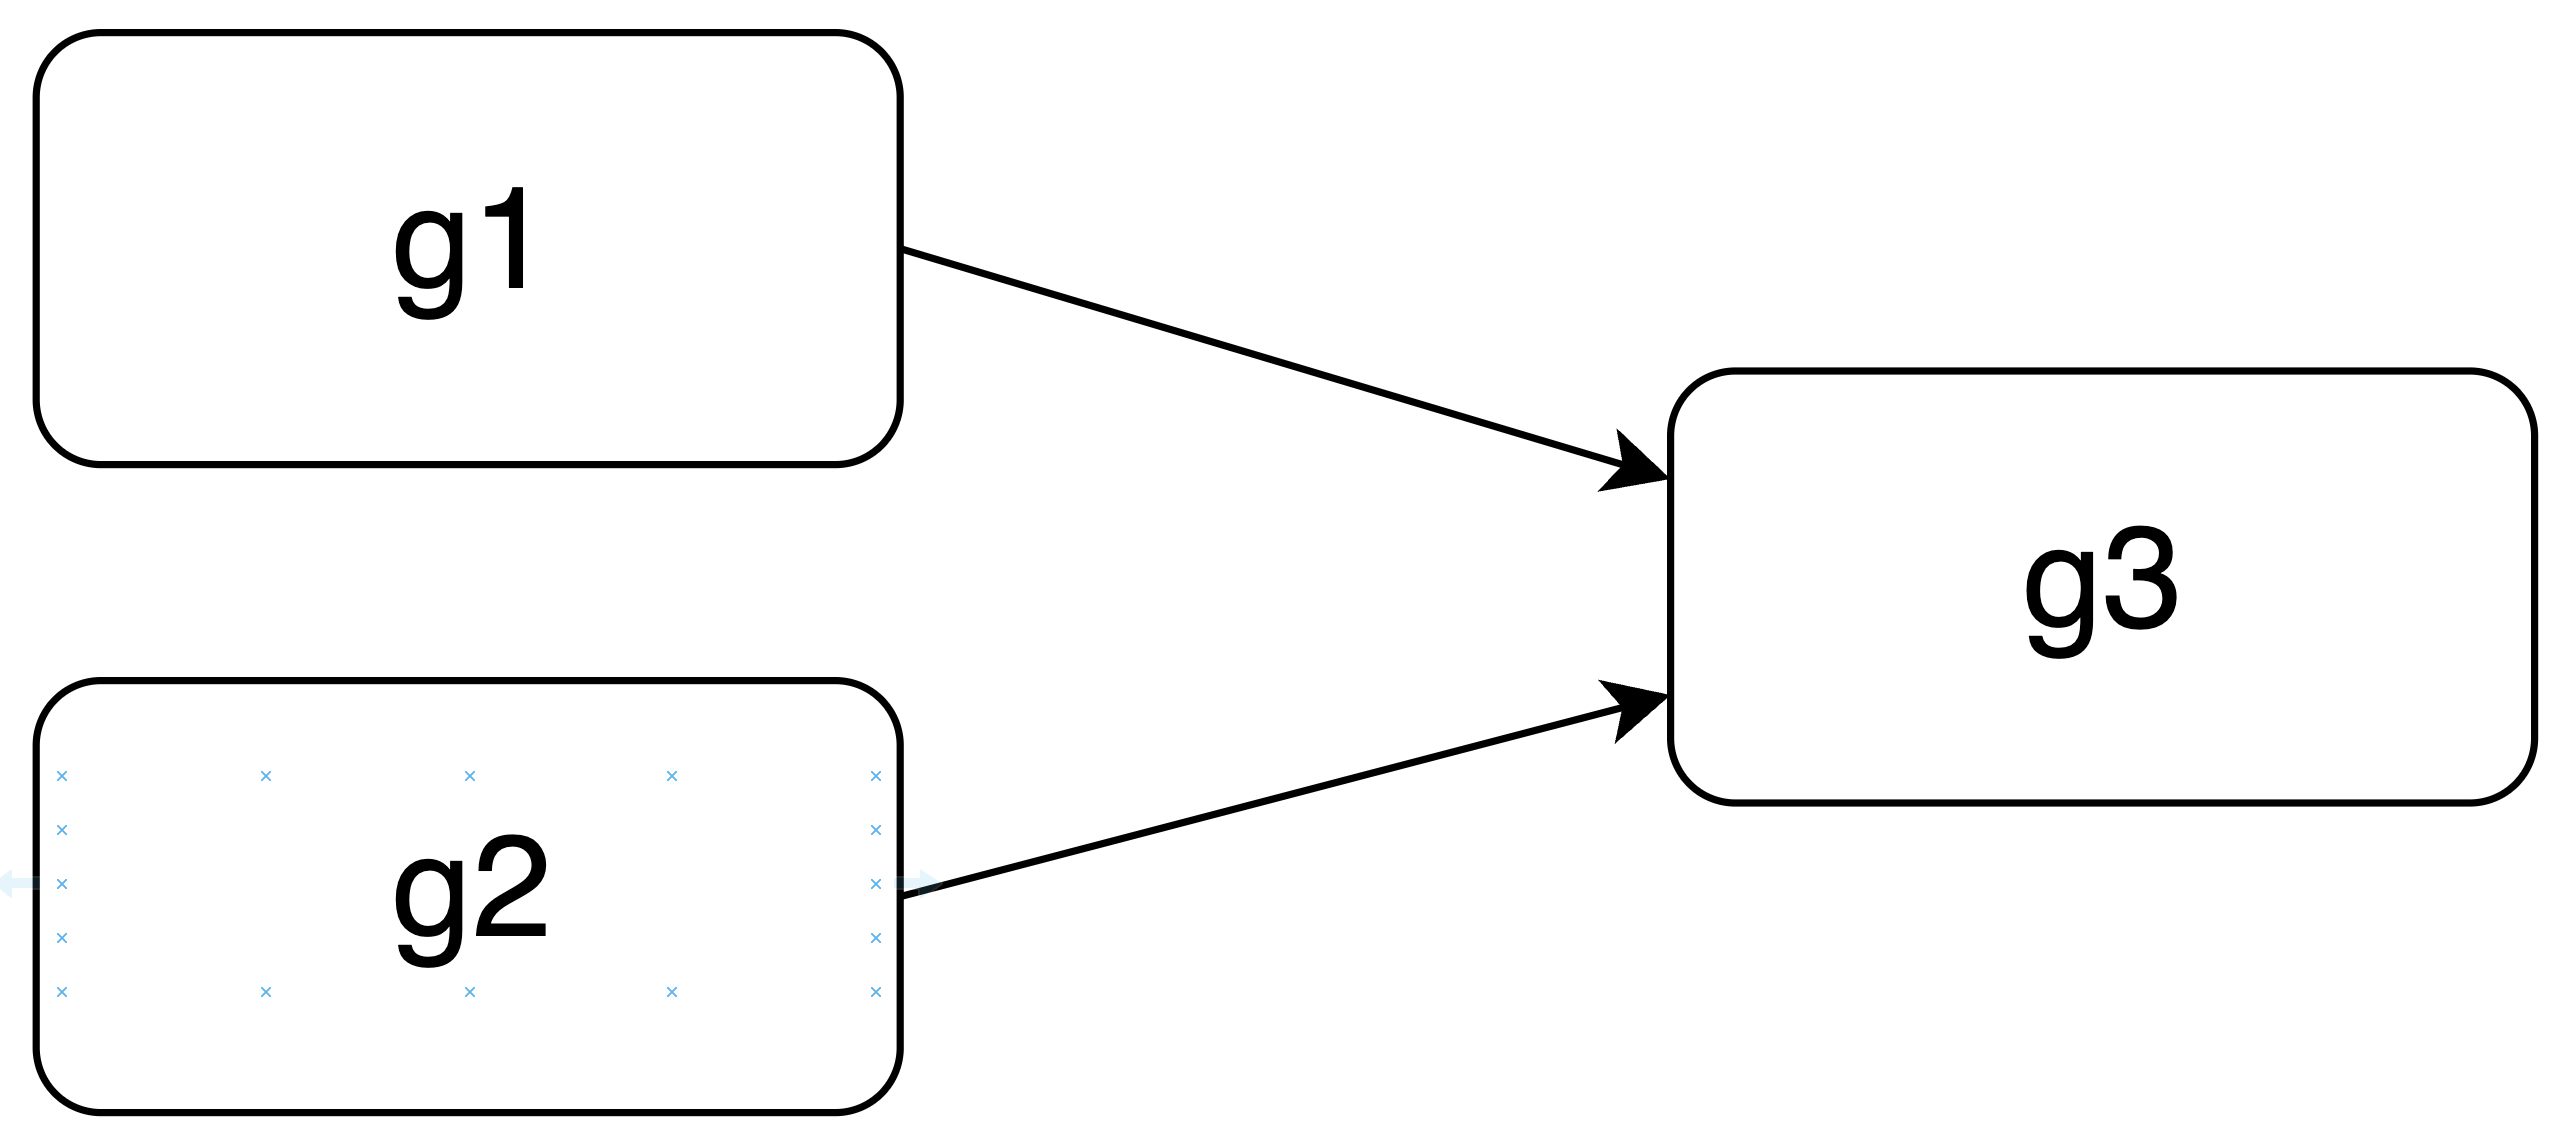
\includegraphics[width=0.9\textwidth]{images/visual-language/dependency-and.png}
        \caption{Dependency between goals with \texttt{AND} semantics.}
        \label{fig:dependency-and}
    \end{subfigure}
    \begin{subfigure}[h]{0.5\linewidth}
        \centering
        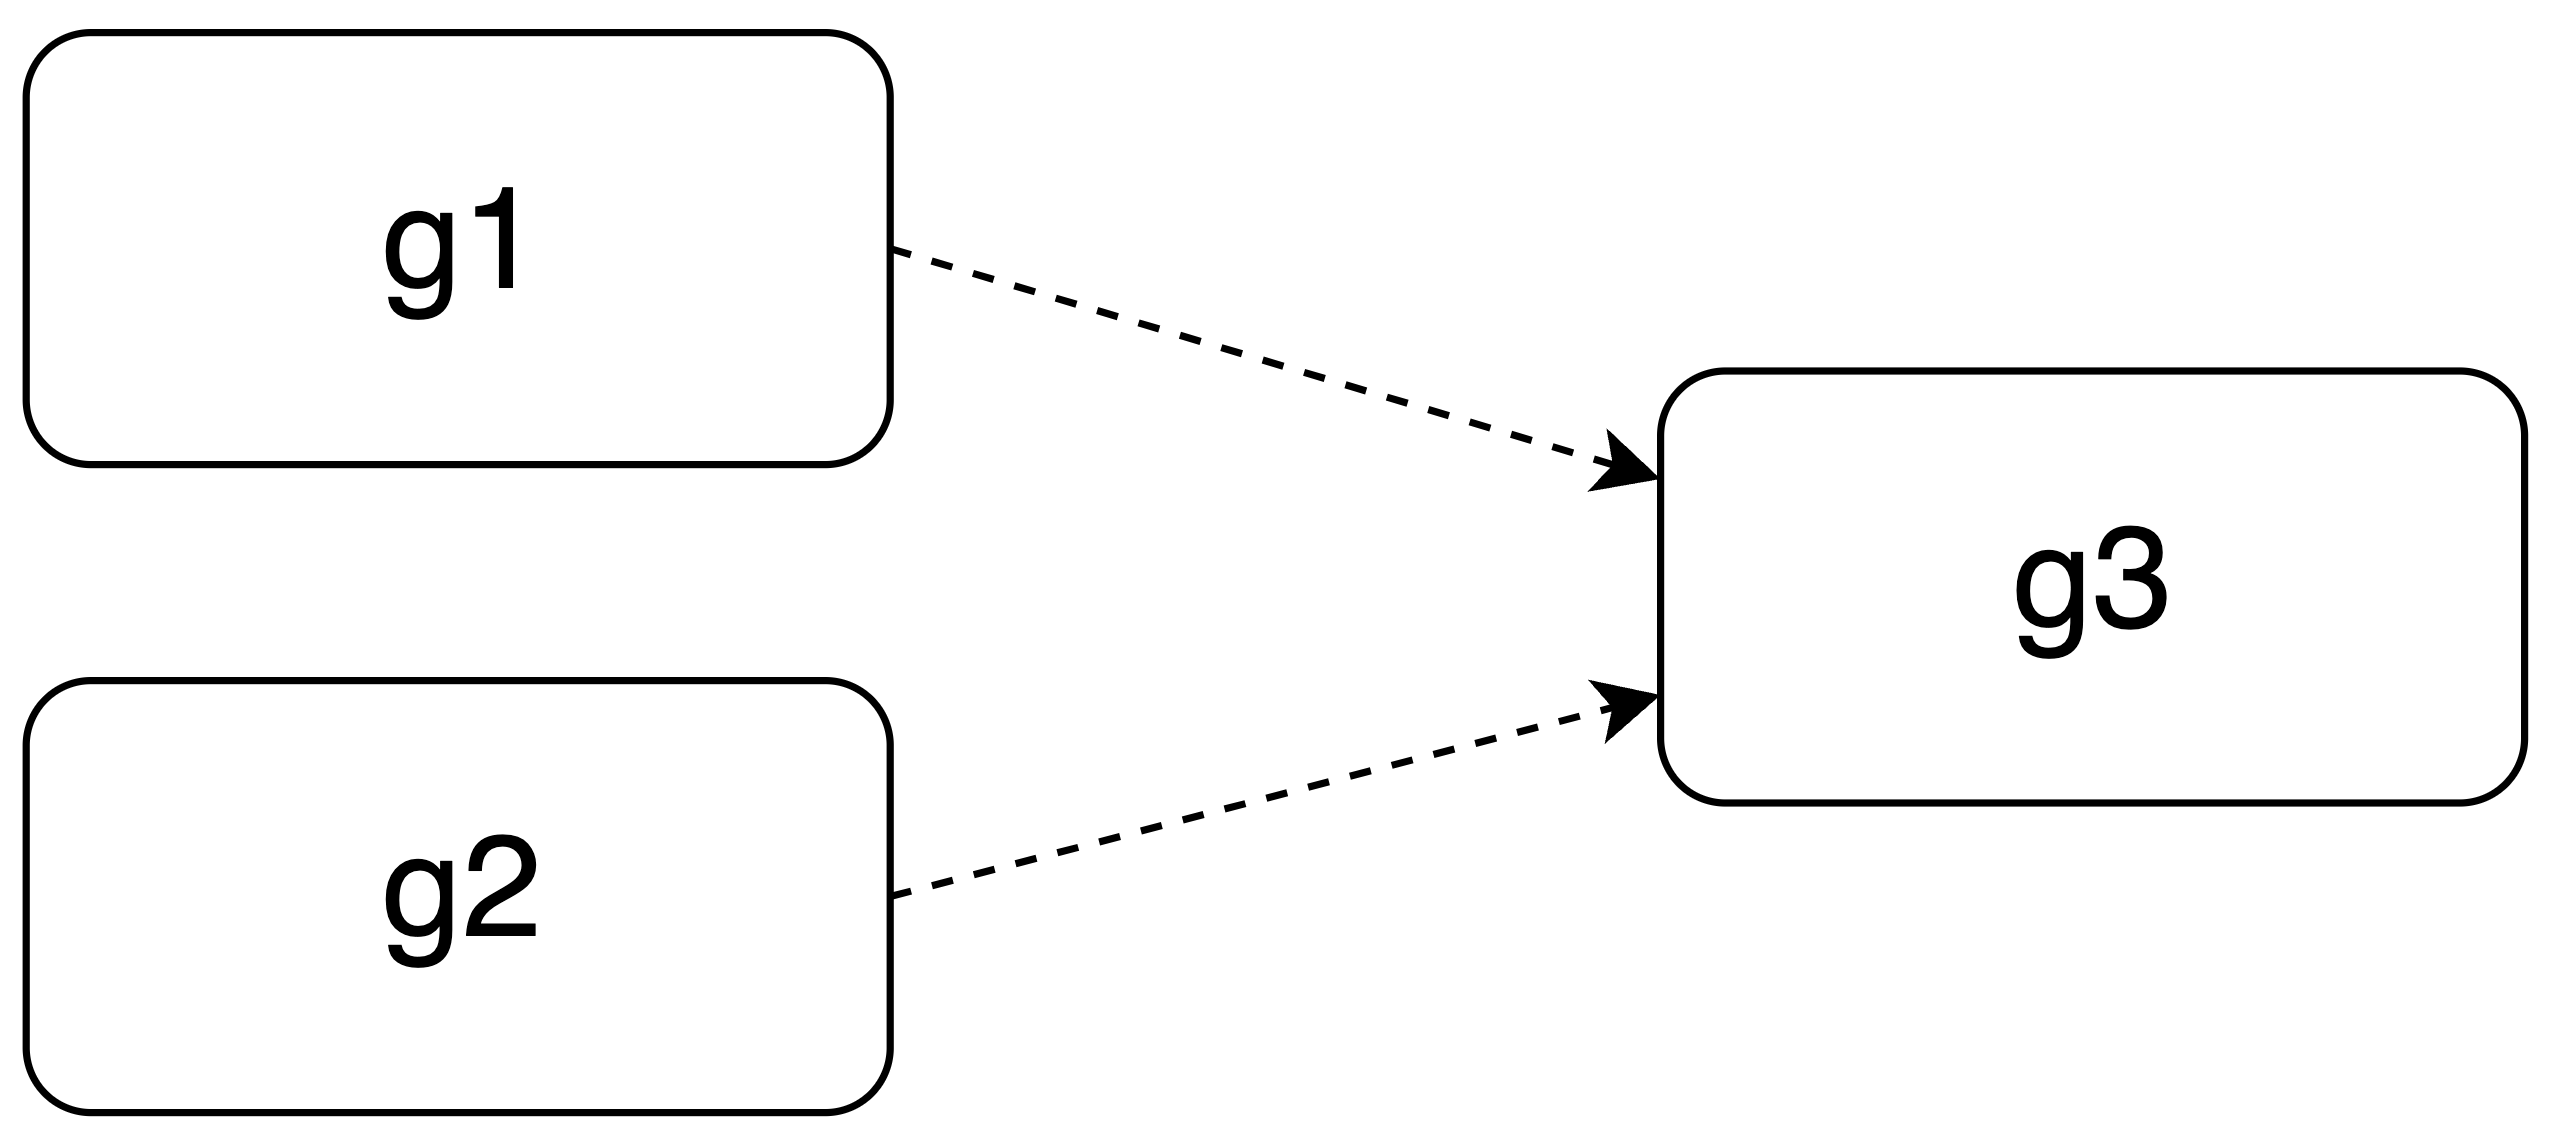
\includegraphics[width=0.9\textwidth]{images/visual-language/dependency-or.png}
        \caption{Dependency between goals with \texttt{OR} semantics.}
        \label{fig:dependency-or}
    \end{subfigure}
    \caption{Visual representation of the dependencies among goals.}
    \label{fig:dependencies}
\end{figure}

It is possible to define two types of dependencies between goals with different semantics.

The first type of dependency is the \textit{AND} dependency, visible in \cref{fig:dependency-and}, which is represented by an arrow with a solid line and a harrow head on the target end.
In this scenario, the target goal \texttt{g3} depends on the source goals \texttt{g1} and \texttt{g2}.
The \texttt{AND} semantics means that the target goal can be achieved only if all the source goals are achieved, with similar behavior to the plan with \texttt{parallel} operator in \moise{}.

$$g3 = g1 \wedge g2$$

On the other hand, the second type of dependency is the \textit{OR} dependency, depicted in \cref{fig:dependency-or}, which is represented by an arrow with a dashed line and a harrow head on the target end. In this scenario, the target goal \texttt{g3} depends on the source goals \texttt{g1} and \texttt{g2}. The \texttt{OR} semantics means that the target goal can be achieved if at least one of the source goals is achieved, with similar behavior to the plan with \texttt{choice} operator in \moise{}.

$$g3 = g1 \vee g2$$

Finally, the \texttt{sequence} operator is achieved through the concept of dependency itself, since dependencies have a \textit{finish-to-start} relationship, meaning that the target goal can be achieved only after the source goals are achieved.

The dependency graph closely resembles the concept of a \textit{Program Evaluation and Review Technique (PERT) diagram}~\cite{donald1972}, which is a statistical tool used in project management designed to analyze and represent the tasks involved in completing a given project.
However, unlike the latter which is usually made up of a single connected component, the dependency graph here described explicitly allows the user to define multiple connected components to represent groups of goals that can be achieved independently.

\subsubsection{Goals Allocation}
Although goals allocation in \moise{} is handled through norms in a separate dimension from the structural and functional one, the visual language allows the user to define the allocation of goals to roles directly in the functional specification diagram.
Indeed, having a third diagram to accomplish this task would make the process of defining the organization unnecessarily complex.
Therefore, being the drawbacks in terms of customization negligible, the choice was made to exploit the functional specification diagram.

This choice also abstracts from the concept of \textit{mission} that is no longer needed to define the allocation of goals to roles.
While in \moise{} goals can be grouped to form missions, which are then assigned to roles, in the visual language the goals are directly assigned to roles without the need for an intermediate step.
Again, the ease of use and the simplicity of the diagram were preferred over the possibility of customization, which is acceptable in most actual use cases.

The role responsible for achieving a goal is represented by a circle with the initials of the role's name written inside it.
To represent that a role is responsible for achieving a goal, its circle is placed inside the rectangle representing the goal, as shown in \cref{fig:goal-allocation}.

\begin{figure}[H]
    \centering
    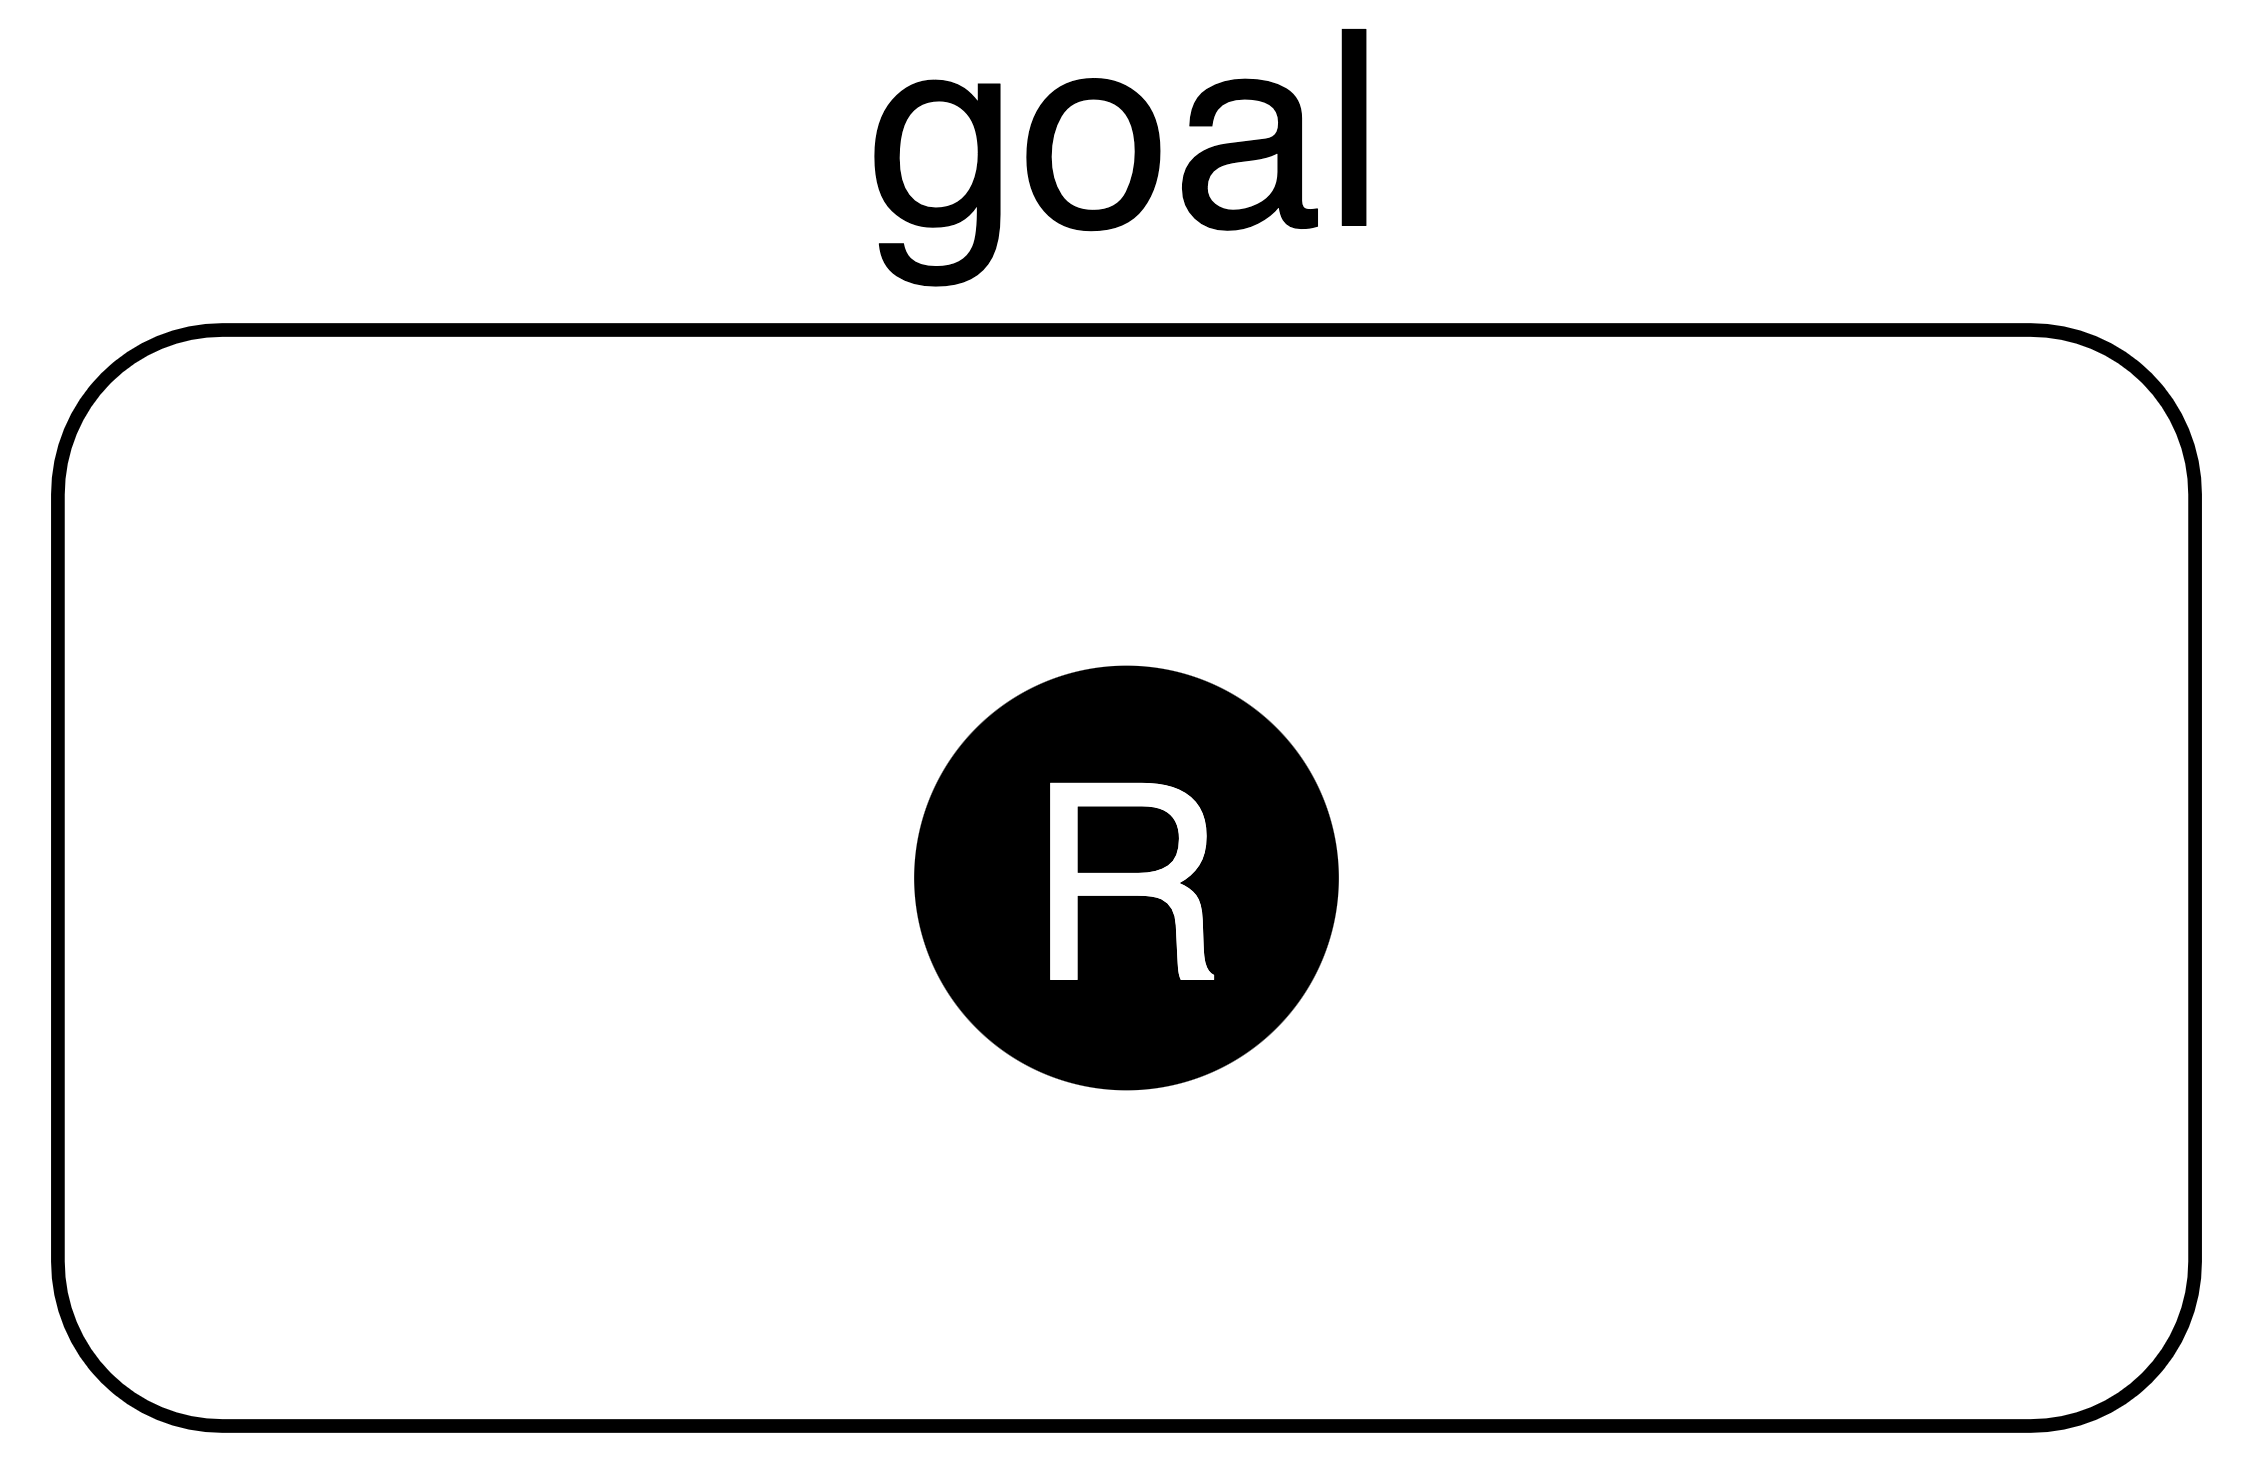
\includegraphics[width=0.3\linewidth]{images/visual-language/goal-allocation.png}
    \caption{Representation of a goal allocation.}
    \label{fig:goal-allocation}
\end{figure}

The visual representation of the rectangle corresponding to the goal slightly changes when a role is responsible for achieving it.
Indeed, the goal name is moved from inside the rectangle to the top of it to make room for the roles.

There are two ways in which a goal can be assigned to a role and they come with different semantics, corresponding to the \textit{deontic modalities} of \moise{}'s normative dimension:
\begin{itemize}
    \item \textbf{Obligation}: the goal is assigned to the role with the \texttt{obligation} modality, meaning that the agent playing that role is obliged to achieve the goal.
    \item \textbf{Permission}: the goal is assigned to the role with the \texttt{permission} modality, meaning that the agent playing that role is allowed to achieve the goal if it wants to.
\end{itemize}

As far as the cardinality of goal allocation is concerned, multiple scenarios are possible.
A goal can be assigned to one, multiple, or no roles.

When the goal is assigned to no roles, it means that no specific agent will actively achieve it, but the goal will be considered as achieved as soon as the goals it depends on are achieved.
This is particularly useful when representing dummy goals that are used to represent the completion of a task.
Indeed, they improve the readability and understandability of the diagram but do not affect the actual behavior of the organization.

Moreover, the type of role that the goal is assigned to slightly changes the semantics.
If the goal is assigned to a \textit{concrete} role, then the goal is assigned to that specific role.
On the other hand, if the goal is assigned to an \textit{abstract} role, then the goal can be assigned to all the roles that are instances of, i.e. extend from, that abstract role.


\section{Main Components and Architecture}
During the design process, it was also necessary to identify all the software components that would be needed to address the requirements of the system.
The choice of the components was made trying to optimize the separation of responsibilities and to minimize the coupling between the different components, thus obtaining a clean and expandable architecture.

\subsection{Web-based IDE}
This component represents the front end and it is the main interface through which the user interacts with the system.

As already mentioned, the Web-based IDE allows the users to create and edit the organization specifications through a user-friendly and intuitive graphical interface.
Specifically, since the designed visual language includes two diagrams, the IDE provides the user with two different views to edit the structural and functional diagrams, respectively.

What is more, the IDE is also responsible for the translation of the organization specifications from the visual language to a format that can be understood by the JaCaMo platform.
In particular, the translation happens from and to the XML format, which is the format used to represent the organization specification in \moise{}.
This allows the user to easily import and export the specifications.

Finally, the IDE provides the user with the possibility to run the organization created and enforce it on the agents currently running in the runtime environment.
Therefore, the component includes an additional view that allows the user to directly interact with the agents.

\subsection{Storage \& Backend}
Since the user should be able to save the organization specifications and load them later, the system needs a component that is responsible for the persistence of the data.
This component should therefore provide basic CRUD functionalities for the organization specifications.

Since the data to be stored is not very complex and structured, but rather consists of strings representing the XML files, the choice was made to use a NoSQL database.
In particular, the choice fell on a document-oriented database because of its simplicity and the fact that it is possible to define flexible schemas that allow for the data model to evolve as applications need change.

Together with the storage component, the system also includes a \textit{backend}.
The latter has a twofold purpose:
\begin{itemize}
    \item It serves as a proxy between the Web-based IDE and the storage component, thus hiding the details of the storage mechanism from the IDE.
    \item It provides an URL to the runtime environment through which the latter can retrieve the organizations' files.
\end{itemize}
To achieve the above goals, the backend component exposes an HTTP API.
This approach allows the Web-based IDE to perform operations on the stored data in a REST-like fashion and the runtime environment to retrieve organization specifications treated as resources, therefore adhering to the Web architecture.

\subsection{Runtime Environment}
This component is responsible for the execution of a MAS and therefore hosts the agents that are currently running.
Thus, it will be also in charge of keeping track of the runtime information about the organizations and making the agents aware of them.
In order for the organization to be enforced on the agents, the Web-based IDE needs to communicate with the runtime environment and send the organization entities to it.

What is more, the Web-based IDE also needs to be able to retrieve information about the running agents so that users can directly assign roles to them when specifying the organization entities.

Finally, the runtime environment should communicate with the backend component in order to retrieve the organization specifications files using URLs.
URLs are provided by the Web-based IDE when the latter sends an organization entity to the runtime environment.

\begin{figure}
    \centering
    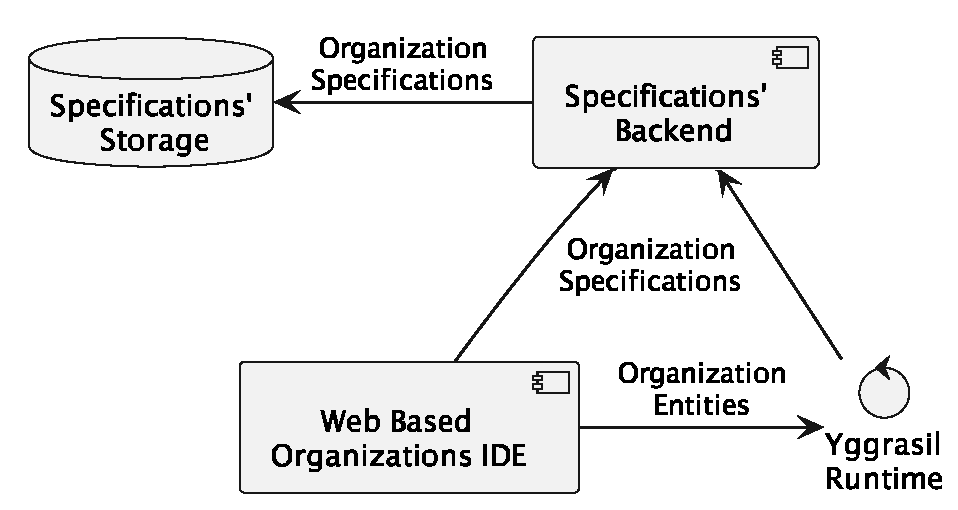
\includegraphics[width=0.8\linewidth]{images/architecture.eps}
    \caption{Overall architecture of the system.}
    \label{fig:architecture}
\end{figure}